\chapter{动态规划}
如果一个问题具有以下两个要素:
\begindot
\item 最优子结构(optimal substructure)
\item 重叠子问题(overlap subproblem)
\myenddot
则可以用动态规划求最优解。

动态规划分为4个步骤:
\begindot
\item 描述最优解的结构。即抽象出一个状态来表示最优解。
\item 递归的定义最优解的值。找出状态转移方程,然后递归的定义
\item 计算最优解的值。典型的做法是自底向上,当然也可以自顶向下。
\item 根据计算过程中得到的信息,构造出最优解。如果我们只需要最优解的值,不需要最
优解本身,则可以忽略第4步。当执行第4步时,我们需要在第3步的过程中维护一些额外的
信息,以便我们能方便的构造出最优解。
\myenddot
在第1步中,我们需要抽象出一个“状态”,在第2步中,我们要找出“状态转移方程”,然后才能
递归的定义最优解的值。第3步和第4步就是写代码实现了。

写代码实现时有两种方式,“递归(recursive)+自顶向下(top-down)+表格(memoization)”和
“自底向上(bottom-up)+表格”。自顶向下也称为记忆化搜索,自底向上也称为递推(不是递归)。

动规用表格将各个子问题的最优解存起来,避免重复计算,是一种空间换时间。

动规与贪心的相同点:最优子结构。

不同点:1、动规的子问题是重叠的,而贪心的子问题是不重叠的(disjoint subproblems);
2、动规不具有贪心选择性质;3、贪心的前进路线是一条线,而动规是一个DAG。

分治和贪心的相同点:disjoint subproblems。


\section{最长公共子序列} %%%%%%%%%%%%%%%%%%%%%%%%%%%%%%
\subsubsection{描述}
一个序列的子序列(subsequence)是指在该序列中删去若干(可以为0个)元素后得到的序列。
准确的说,若给定序列$X=(x_1,x_2,\cdots,x_m)$,则另一个序列$Z=(z_1,z_2,\cdots,z_k)$,
是X的子序列是指存在一个严格递增下标序列$(i_1,i_2,\cdots,i_k)$使得对于所有$j=1,2,\cdots,k$
有$z_j=x_{i_j}$。例如,序列$Z=(B,C,D,B)$是序列$X=(A,B,C,B,D,A,B)$的子序列,相应的
递增下标序列为$(1,2,4,6)$。

给定两个序列X和Y,求X和Y的最长公共子序列(longest common subsequence)。

\subsubsection{输入}
输入包括多组测试数据,每组数据占一行,包含两个字符串(字符串长度不超过200),代表两个序列。
两个字符串之间由若干个空格隔开。

\subsubsection{输出}
对每组测试数据,输出最大公共子序列的长度,每组一行。

\subsubsection{样例输入}
\begin{Code}
abcfbc abfcab
programming contest 
abcd mnp
\end{Code}

\subsubsection{样例输出}
\begin{Code}
4
2
0
\end{Code}

\subsubsection{分析}
最长公共子序列问题具有最优子结构性质。
设序列$X=(x_1,x_2,\cdots,x_m)$和$Y=(y_1,y_2,\cdots,y_n)$的最长公共子序列为$Z=(z_1,z_2,\cdots,z_k)$,则
\begindot
\item 若$x_m=y_n$,则$z_k=x_m=y_n$,且$Z_{k-1}$是$X_{m-1}$和$Y_{n-1}$的最长公共子序列。
\item 若$x_m \neq y_n$且$z_k \neq x_m$,则Z是$X_{m-1}$和$Y$的最长公共子序列。
\item 若$x_m \neq y_n$且$z_k \neq y_n$,则Z是$X$和$Y_{n-1}$的最长公共子序列。
\myenddot
其中,$X_{m-1}=(x_1,x_2,\cdots,x_{m-1})$, $Y_{n-1}=(y_1,y_2,\cdots,y_{n-1})$, $Z_{k-1}=(z_1,z_2,\cdots,z_{k-1})$。

设状态为d[i][j],表示序列$X_i$和$Y_j$的最长公共子序列的长度。由最优子结构可得状态转移方程如下:
$$
d[i][j]=\begin{cases}
0 & i=0,j=0\\
d[i-1][j-1]+1 & i,j>0; x_i=y_i \\
\max\left\{d[i][j-1],d[i-1][j]\right\} & i,j>0; x_i \neq y_i
\end{cases}
$$

如果要打印出最长公共子序列,需要另设一个数组p,p[i][j]记录d[i][j]是由哪个子问题得到的。

\subsubsection{代码}
\begin{Codex}[label=lcs.c]
#include <stdio.h>
#include <string.h>

#define MAX 201  /* 字符串最大长度为200 */

int d[MAX][MAX]; /* d[i][j]表示序列Xi和Yj的最长公共子序列的长度 */
char x[MAX], y[MAX];  /* 字符串末尾有个'0' */

void lcs(const char *x, const int m, const char *y, const int n) {
    int i, j;
    
    for (i = 0; i <= m; i++) d[i][0] = 0;  /* 边界初始化 */
    for (j = 0; j <= n; j++) d[0][j] = 0;

    for (i = 1; i <= m; i++) {
        for (j = 1; j <= n; j++) {
            if (x[i-1] == y[j-1]) {
                d[i][j] = d[i-1][j-1] + 1;
            } else {
                d[i][j] = d[i-1][j] > d[i][j-1] ? d[i-1][j] : d[i][j-1];
            }
        }
    }
}

void lcs_extend(const char *x, const int m, const char *y, const int n);
void lcs_print(const char *x, const int m, const char *y, const int n);

int main() {
    /* while (scanf ("%s%s", a, b)) { /* TLE */
    /* while (scanf ("%s%s", a, b) == 2) {  /* AC */
    while (scanf ("%s%s", x, y) != EOF) { /* AC */
        const int lx = strlen(x);
        const int ly = strlen(y);
        lcs(x, lx, y, ly);
        printf ("%d\n", d[lx][ly]);
        /*
        lcs_extend(x, lx, y, ly);
        lcs_print(x, lx, y, ly);
        printf("\n"); */
    }
    return 0;
}

int p[MAX][MAX]; /* p[i][j]记录d[i][j]是由哪个子问题得到的 */

void lcs_extend(const char *x, const int m, const char *y, const int n) {
    int i, j;
    
    memset(p, 0, sizeof(p));
    for (i = 0; i <= m; i++) d[i][0] = 0;  /* 边界初始化 */
    for (j = 0; j <= n; j++) d[0][j] = 0;

    for (i = 1; i <= m; i++) {
        for (j = 1; j <= n; j++) {
            if (x[i-1] == y[j-1]) {
                d[i][j] = d[i-1][j-1] + 1;
                p[i][j] = 1;
            } else {
                if (d[i-1][j] >= d[i][j-1]) {
                    d[i][j] = d[i-1][j];
                    p[i][j] = 2;
                } else {
                    d[i][j] = d[i][j-1];
                    p[i][j] = 3;
                }
            }
        }
    }
}

void lcs_print(const char *x, const int m, const char *y, const int n) {
    if (m == 0 || n == 0) return;

    if (p[m][n] == 1) {
        lcs_print(x, m - 1, y, n - 1);
        printf("%c", x[m - 1]);
    } else if (p[m][n] == 2) {
        lcs_print(x, m - 1, y, n);
    } else {
        lcs_print(x, m, y, n - 1);
    }
}
\end{Codex}

\subsubsection{相关的题目}
与本题相同的题目:
\begindot
\item 《计算机算法设计与分析(第3版)》\footnote{王晓东, 计算机算法设计与分析(第3版), 电子工业出版社, 2007}第56页3.3节
\item POJ 1458 Common Subsequence, \myurl{http://poj.org/problem?id=1458}
\item HDOJ 1159 Common Subsequence, \myurl{http://acm.hdu.edu.cn/showproblem.php?pid=1159}
\item 《程序设计导引及在线实践》\footnote{李文新,程序设计导引及在线实践, 清华大学出版社, 2007}第203页10.5节
\item 百练 2806 公共子序列, \myurl{http://poj.grids.cn/practice/2806/}
\myenddot

与本题相似的题目:
\begindot
\item HDOJ 1080 Human Gene Functions, \myurl{http://acm.hdu.edu.cn/showproblem.php?pid=1080}
\item HDOJ 1503 Advanced Fruits, \myurl{http://acm.hdu.edu.cn/showproblem.php?pid=1503}
\myenddot


\section{最大连续子序列和} %%%%%%%%%%%%%%%%%%%%%%%%%%%%%%
\subsubsection{描述}
给定一个整数序列$S_1,S_2,\cdot,S_n(1 \leq n \leq 1,000,000, -32768 \leq S_i \leq 32768)$,定义函数$sum(i,j)=S_i+\cdot+S_j(1 \leq i \leq j \leq n)$。

求最大的$sum(i,j)$,即\textbf{最大连续子序列和}(maximum continuous subsequence sum)。

\subsubsection{输入}
每个测试用例由正整数n开头,接着是n个整数。

\subsubsection{输出}
每行输出一个最大和。

\subsubsection{样例输入}
\begin{Code}
3 1 2 3
6 -1 4 -2 3 -2 3
\end{Code}

\subsubsection{样例输出}
\begin{Code}
6
6
\end{Code}

\subsubsection{分析}
设状态为d[j],表示以S[j]结尾的最大连续子序列和,则状态转移方程如下:
\begin{eqnarray}
d[j] &=& \max\left\{d[j-1]+S[j],S[j]\right\}, \text{ 其中 }1 \leq j \leq n \nonumber \\
target &=& \max\left\{d[j]\right\}, \text{ 其中 }1 \leq j \leq n \nonumber
\end{eqnarray}

解释如下:
\begindot
\item 情况一,S[j]不独立,与前面的某些数组成一个连续子序列,则最大连续子序列和为$d[j-1]+S[j]$。
\item 情况二,S[j]独立划分成为一段,即连续子序列仅包含一个数S[j],则最大连续子序列和为$S[j]$。
\myenddot    

\subsubsection{代码}
\begin{Codex}[label=mcss.c]
#include <stdio.h>
#include <stdlib.h>

inline static int max(int a , int b) {
   return (a > b) ? a : b ;
}

inline static int min(int a , int b) {
   return (a < b) ? a : b ;
}

/**
 * @brief 最大连续子序列和,思路四
 * @param[in] S 数列
 * @param[in] n 数组的长度
 * @return 最大连续子序列和
 */
int mcss(int S[], int n) {
    int i, maxs, mins;
    int *sum = (int*) malloc((n + 1) * sizeof(int));  // 前n项和
    sum[0] = 0;
    maxs = 0, mins = 0;
    for (i = 1; i <= n; i++) {
        sum[i] = sum[i - 1] + S[i - 1];
        maxs = max(maxs, sum[i]);
        mins = min(mins, sum[i]);
    }
    free(sum);
    return maxs - mins;
}

/**
 * @brief 最大连续子序列和,动规
 * @param[in] S 数列
 * @param[in] n 数组的长度
 * @return 最大连续子序列和
 */
int mcss_dp(int S[], int n) {
    int i, result;
    int *d = (int*) malloc(n * sizeof(int));
    d[0] = S[0];
    result = d[0];
    for (i = 1; i < n; i++) {
        d[i] = max(S[i], d[i - 1] + S[i]);
        if (result < d[i])
            result = d[i];
    }
    free(d);
    return result;
}

int main() {
    int n, *S;
    while (scanf("%d", &n) > 0) {
        int i;
        S = (int*) malloc(n * sizeof(int));
        for (i = 0; i < n; i++)
            scanf("%d", &S[i]);

        printf("%d\n", mcss_dp(S, n));
        free(S);
    }
    return 0;
}
\end{Codex}

\subsubsection{其他解法}

\begindot
\item 思路一:直接在i到j之间暴力枚举,复杂度是$O(n^3)$
\item 思路二:处理后枚举,连续子序列的和等于两个前缀和之差,复杂度$O(n^2)$。
\item 思路三:分治法,把序列分为两段,分别求最大连续子序列和,然后归并,复杂度$O(n\log n)$
\item 思路四:把$O(n^2)$的代码稍作处理,得到$O(n)$的算法
\item 思路五:M=1的最大M子段和,见第 \S \ref{sec:mmss} 节
\myenddot

感兴趣的读者请参考这篇博客,\myurl{http://www.cnblogs.com/gj-Acit/archive/2013/02/12/2910332.html}

\subsubsection{相关题目}
与本题相同的题目:
\begindot
\item TODO
\myenddot

与本题相似的题目:
\begindot
\item HDOJ 1024 Max Sum Plus Plus, \myurl{http://acm.hdu.edu.cn/showproblem.php?pid=1024}
\myenddot


\section{最大M子段和} %%%%%%%%%%%%%%%%%%%%%%%%%%%%%%
\label{sec:mmss}

\subsubsection{描述}
给定一个整数序列$S_1,S_2,\cdot,S_n(1 \leq n \leq 1,000,000, -32768 \leq S_i \leq 32768)$,定义函数$sum(i,j)=S_i+ ... +S_j(1 \leq i \leq j \leq n)$。

现给定一个正整数m,找出m对i和j,使得$sum(i_1,j_1)+sum(i_2,j_2)+ ... +sum(i_m,j_m)$最大。这就是\textbf{最大M子段和}(maximum m segments sum)。

\subsubsection{输入}
每个测试用例由两个正整数m和n开头,接着是n个整数。

\subsubsection{输出}
每行输出一个最大和。

\subsubsection{样例输入}
\begin{Code}
1 3 1 2 3
2 6 -1 4 -2 3 -2 3
\end{Code}

\subsubsection{样例输出}
\begin{Code}
6
8
\end{Code}

\subsubsection{分析}
设状态为d[i,j],表示前j项分为i段的最大和,且第i段必须包含S[j],则状态转移方程如下:
\begin{eqnarray}
d[i,j] &=& \max\left\{d[i,j-1]+S[j],\max\left\{d[i-1,t]+S[j]\right\}\right\}, \text{ 其中 }i \leq j \leq n, i-1 \leq t < j \nonumber \\
target &=& \max\left\{d[m,j]\right\}, \text{ 其中 }m \leq j \leq n \nonumber
\end{eqnarray}

分为两种情况:
\begindot
\item 情况一,S[j]包含在第i段之中,$d[i,j-1]+S[j]$。
\item 情况二,S[j]独立划分成为一段,$\max\left\{d[i-1,t]+S[j]\right\}$。
\myenddot

观察上述两种情况可知d[i,j]的值只和d[i,j-1]和d[i-1,t]这两个值相关,因此不需要二维数组,可以用滚动数组,只需要两个一维数组,用d[j]表示现阶段的最大值,即$d[i,j-1]+S[j]$,用prev[j]表示上一阶段的最大值,即$\max\left\{d[i-1,t]+S[j]\right\}$。

\subsubsection{代码}
\begin{Codex}[label=mmss.c]
#include <stdio.h>
#include <stdlib.h>
#include <limits.h>

/**
 * @brief 最大m段子序列和
 * @param[in] S 数组
 * @param[in] n 数组长度
 * @param[in] m m段
 * @return 最大m段子序列和
 */
int mmss(int S[], int n, int m) {
    int max_sum, i, j;

    /* d[i]表示现阶段最大值,prev[i]表示上阶段最大值 */
    /* d[0], prev[0] 未使用 */
    int *d = (int*) calloc(n + 1, sizeof(int));
    int *prev = (int*) calloc(n + 1, sizeof(int));
    S--;  // 因为 j是从1开始,而S从0开始,这里要减一

    for (i = 1; i <= m; ++i) {
        max_sum = INT_MIN;
        for (j = i; j <= n; ++j) {
            // 状态转移方程
            if (d[j - 1] < prev[j - 1])
                d[j] = prev[j - 1] + S[j];
            else
                d[j] = d[j - 1] + S[j];

            prev[j - 1] = max_sum;  // 存放上阶段最大值
            if (max_sum < d[j])
                max_sum = d[j];  // 更新 max_sum
        }
        prev[j - 1] = max_sum;
    }

    free(d);
    free(prev);
    return max_sum;
}

int main() {
    int n, m, i, *S;
    while (scanf("%d%d", &m, &n) == 2) {
        S = (int*) malloc(sizeof(int) * n);
        for (i = 0; i < n; ++i)
            scanf("%d", &S[i]);
        printf("%d\n", mmss(S, n, m));
        free(S);
    }
    return 0;
}
\end{Codex}

\subsubsection{相关题目}
与本题相同的题目:
\begindot
\item HDOJ 1024 Max Sum Plus Plus, \myurl{http://acm.hdu.edu.cn/showproblem.php?pid=1024}
\myenddot

与本题相似的题目:
\begindot
\item LeetCode Best Time to Buy and Sell Stock III, \myurl{http://leetcode.com/onlinejudge\#question_123},\\
参考代码\myurl{https://gist.github.com/soulmachine/5906637}
\myenddot


\section{DAG上的动态规划} %%%%%%%%%%%%%%%%%%%%%%%%%%%%%%

\subsection{数字三角形}

\subsubsection{描述}
有一个由非负整数组成的三角形,第一行只有一个数,除了最下一行之外每个数的左下角和右下
角各有一个数,如图~\ref{fig:numbersTriangle}所示。

\begin{center}
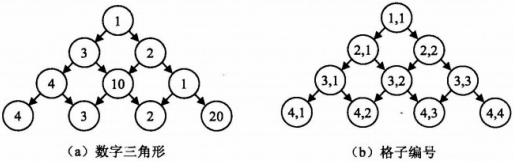
\includegraphics[width=360pt]{numbers-triangle.png}\\
\figcaption{数字三角形问题}\label{fig:numbersTriangle}
\end{center}

从第一行的数开始,每次可以往左下或右下走一格,直到走到最下行,把沿途经过的数全部加起来。
如何走才能使得这个和最大?

\subsubsection{输入}
第一行是一个整数$N (1 \le N \leq 100)$,给出三角形的行数。接下来的N行给出数字三角形。三
角形中的数全部是整数,范围在0到100之间。

\subsubsection{输出}
输出最大的和。

\subsubsection{样例输入}
\begin{Code}
5
7
3 8 
8 1 0  
2 7 4 4 
4 5 2 6 5
\end{Code}

\subsubsection{样例输出}
\begin{Code}
30
\end{Code}

\subsubsection{分析}
这是一个动态决策问题,在每层有两种选择,左下或右下,因此一个n层的数字三角形有$2^n$条路线。

可以用回溯法,用回溯法求出所有可能的路线,就可以从中选出最优路线。但是由于有$2^n$条路线,
回溯法很慢。

本题可以用动态规划来求解(具有最有子结构和重叠子问题两个要素,后面会看到)。把当前位置(i,j)看
成一个状态,然后定义状态d[i][j]为从位置(i,j)出发时能得到的最大和(包括格子(i,j)本
身的值a[i][j])。在这个状态定义下,原问题的解是d[0][0]。

下面来看看不同状态之间是怎样转移的。从位置(i,j)出发有两种决策,如果往左走,则走到(i+1,j)后需要求
“从(i+1,j)出发后能得到的最大和”这一子问题,即d[i+1][j],类似地,往右走之后需要求d[i+1][j+1]。应该
选择d[i+1][j]和d[i+1][j+1]中较大的一个,因此可以得到如下的状态转移方程:
$$d[i][j]=a[i][j]+\max\left\{d[i+1][j], d[i+1][j+1]\right\}$$

\subsubsection{代码}
版本1,自顶向下。

\begin{Codex}[label=numbers_triangle1.c]
#include<stdio.h>
#include<string.h>

#define MAXN 100

int n, a[MAXN][MAXN], d[MAXN][MAXN];

int max(const int x, const int y) {
    return x > y ? x : y;
}

/**
 * @brief 求从位置(i,j)出发时能得到的最大和
 * @param[in] i 行
 * @param[in] j 列
 * @return 最大和
 */
int dp(const int i, const int j) {
    if(d[i][j] >= 0) {
        return d[i][j];
    } else {
        return d[i][j] = a[i][j] + (i == n-1 ? 0 : max(dp(i+1, j+1), dp(i+1, j)));
    }
}

int main() {
    int i, j;
    memset(d, -1, sizeof(d));

    scanf("%d", &n);
    for(i = 0; i < n; i++)
      for (j = 0; j <= i; j++) scanf("%d", &a[i][j]);
    
    printf("%d\n", dp(0, 0));
    return 0;
}
\end{Codex}

版本2,自底向上。

\begin{Codex}[label=numbers_triangle2.c]
#include<stdio.h>
#include<string.h>

#define MAXN 100

int n, a[MAXN][MAXN], d[MAXN][MAXN];

int max(const int x, const int y) {
    return x > y ? x : y;
}

/**
 * @brief 自底向上计算所有子问题的最优解
 * @return 无
 */
void dp() {
    int i, j;
    for (i = 0; i < n; ++i) {
        d[n-1][i] = a[n-1][i];
    }
    for (i = n-2; i >= 0; --i)
      for (j = 0; j <= i; ++j)
        d[i][j] = a[i][j] + max(d[i+1][j], d[i+1][j+1]);
}

int main() {
    int i, j;
    memset(d, -1, sizeof(d));

    scanf("%d", &n);
    for(i = 0; i < n; i++)
      for (j = 0; j <= i; j++) 
          scanf("%d", &a[i][j]);

    dp();
    
    printf("%d\n", d[0][0]);
    return 0;
}
\end{Codex}

\subsubsection{相关的题目}
与本题相同的题目:
\begindot
\item 《算法竞赛入门经典》\footnote{刘汝佳,算法竞赛入门经典,清华大学出版社,2009}第159页9.1.1节
\item POJ 1163 The Triangle, \myurl{http://poj.org/problem?id=1163}
\item 百练 2760 数字三角形, \myurl{http://poj.grids.cn/practice/2760/}
\myenddot

与本题相似的题目:
\begindot
\item  TODO
\myenddot

\subsection{嵌套矩形}

\subsubsection{描述}
有$n$个矩形,每个矩形可以用$a,b$来描述,表示长和宽。矩形$X(a,b)$可以嵌套在
矩形$Y(c,d)$中当且仅当$a<c,b<d$或者$b<c,a<d$(相当于旋转X90度)。例如
(1,5)可以嵌套在(6,2)内,但不能嵌套在(3,4)中。你的任务是选出尽可能多的
矩形排成一行,使得除最后一个外,每一个矩形都可以嵌套在下一个矩形内。

\subsubsection{输入}
第一行是一个正整数$N(0<N<10)$,表示测试数据组数,
每组测试数据的第一行是一个正正数n,表示该组测试数据中含有矩形的个数$(n<=1000)$
随后的n行,每行有两个数$a,b(0<a,b<100)$,表示矩形的长和宽

\subsubsection{输出}
每组测试数据都输出一个数,表示最多符合条件的矩形数目,每组输出占一行

\subsubsection{样例输入}
\begin{Code}
1
10
1 2
2 4
5 8
6 10
7 9
3 1
5 8
12 10
9 7
2 2
\end{Code}

\subsubsection{样例输出}
\begin{Code}
5
\end{Code}

\subsubsection{分析}
本题实质上是求DAG中不固定起点的最长路径。

设d[i]表示从结点i出发的最长长度,状态转移方程如下:
$$d[i]=\max\left\{d[j]+1|(i,j) \in E\right\}$$

其中,E为边的集合。最终答案是d[i]中的最大值。

\subsubsection{代码}
\begin{Codex}[label=embedded_rectangles.c]
#include <stdio.h>
#include <string.h>

#define MAXN 1000 // 矩形最大个数

int n; // 矩形个数
int G[MAXN][MAXN]; // 矩形包含关系
int d[MAXN]; // 表格

/**
 * @brief 动规,自顶向下.
 * @param[in] i 起点
 * @return 以i为起点,能达到的最长路径
 */
int dp(const int i) {
    int j;
    int *ans= &d[i];
    if(*ans > 0) return *ans;

    *ans = 1;
    for(j = 0; j < n; j++) if(G[i][j]) {
        const int next = dp(j) + 1;
        if(*ans < next) *ans = next;
    }
    return *ans;
}

/**
 * @brief 按字典序打印路径.
 *
 * 如果多个 d[i] 相等,选择最小的i。
 *
 * @param[in] i 起点
 * @return 无
 */
void print_path(const int i) {
    int j;
    printf("%d ", i);
    for(j = 0; j < n; j++) if(G[i][j] && d[i] == d[j] + 1) {
        print_path(j);
        break;
    }
}

int main() {
    int N, i, j;
    int max, maxi;
    int a[MAXN],b[MAXN];

    scanf("%d", &N);
    while(N--) {
        memset(G, 0, sizeof(G));
        memset(d, 0, sizeof(d));

        scanf("%d", &n);
        for(i = 0; i < n; i++) scanf("%d%d", &a[i], &b[i]);

        for(i = 0; i < n; i++)
            for(j = 0; j < n; j++)
                if((a[i] > a[j] && b[i] > b[j]) ||
                    (a[i] > b[j] && b[i] > a[j])) G[i][j] = 1;

        max = 0;
        maxi = -1;
        for(i = 0; i < n; i++) if(dp(i) > max) {
            max = dp(i);
            maxi = i;
        }
        printf("%d\n", max);
        // print_path(maxi);
    }
    return 0;
}
\end{Codex}

\subsubsection{相关的题目}
与本题相同的题目:
\begindot
\item 《算法竞赛入门经典》\footnote{刘汝佳,算法竞赛入门经典,清华大学出版社,2009}第161页9.2.1节
\item  NYOJ 16 嵌套矩形, \myurl{http://acm.nyist.net/JudgeOnline/problem.php?pid=16}
\myenddot

与本题相似的题目:
\begindot
\item  TODO
\myenddot

\subsection{硬币问题}

\subsubsection{描述}
有$n$种硬币,面值为别为$v_1,v_2,v_3,\cdots, v_n$,每种都有无限多。给定非负整数$S$,可以
选取多少个硬币,使得面值和恰好为$S$?输出硬币数目的最小值和最大值。
$1 \leq n \leq 100, 1 \leq S \leq 10000, 1 \leq v_i \leq S$。

\subsubsection{输入}
第1行$n$,
第2行$S$,
第3到$n+2$行为$n$种不同的面值。

\subsubsection{输出}
第1行为最小值,
第2行为最大值。

\subsubsection{样例输入}
\begin{Code}
3
6
1
2
3
\end{Code}

\subsubsection{样例输出}
\begin{Code}
2
6
\end{Code}

\subsubsection{分析}
本题实质上是求DAG中固定终点的最长路径和最短路径。

把每种面值看作一个点,表示“还需要凑足的面值”,则初始状态为S,目标状态为0。若当前状态为i,
每使用一个硬币j,状态便转移到$i-v_j$。

设状态为d[i],表示从节点i出发的最长路径长度,则原问题的解是d[S]。状态转移方程如下:
$$d[i]=\max\left\{d[j]+1,(i,j) \in E\right\}$$

本题还可以看作是完全背包问题(见\S \ref{sec:ukp}节):背包容量为S,背包必须要装满,物品即硬币,每个硬币的费用为面值$v_i$,
价值均为1。求背包中物品的最小价值和最大价值。

\subsubsection{代码}
版本1,自顶向下。

\begin{Codex}[label=coin_change.c]
#include<stdio.h>
#include <string.h>

#define MAXN 100
#define MAXV 10000

/** 硬币面值的种类. */
int n;
/** 要找零的数目. */
int S;
/** 硬币的各种面值. */
int v[MAXN];
/** min[i] 表示面值之和为i的最短路径的长度,max则是最长. */
int min[MAXV + 1], max[MAXV + 1];

/**
 * @brief 最短路径.
 * @param[in] s 面值
 * @return 最短路径长度
 */
int dp1(const int s) { // 最小值
    int i;
    int *ans = &min[s];
    if(*ans != -1) return *ans;
    *ans = 1<<30;
    for(i = 0; i < n; ++i) if(v[i] <= s) {
        const int tmp = dp1(s-v[i])+1;
        *ans = *ans < tmp ? *ans : tmp;
    }
    return *ans;
}

int visited[MAXV + 1];
/**
 * @brief 最长路径.
 * @param[in] s 面值
 * @return 最长路径长度
 */
int dp2(const int s) { //最大值 
    int i;
    int *ans = &max[s];

    if(visited[s]) return max[s];
    visited[s] = 1;

    *ans = -1<<30;
    for(i = 0; i < n; ++i) if(v[i] <= s) {
        const int tmp = dp2(s-v[i])+1;
        *ans = *ans > tmp ? *ans : tmp;
    }
    return *ans;
}

void print_path(const int* d, const int s);

int main() {
    int i;
    scanf("%d%d", &n, &S);
    for(i = 0; i < n; ++i) scanf("%d", &v[i]);

    memset(min, -1, sizeof(min));
    min[0] = 0;
    printf("%d\n", dp1(S));
    // print_path(min, S);

    memset(max, -1, sizeof(max));
    memset(visited, 0, sizeof(visited));
    max[0] = 0; visited[0] = 1;
    printf("%d\n", dp2(S));
    // print_path(max, S);

    return 0;
}

/**
 * @brief 打印路径.
 * @param[in] d 上面的 min 或 min
 * @param[in] s 面值之和
 * @return 无
 */
void print_path(const int* d, const int s) {//打印的是边
    int i;
    for(i = 0; i < n; ++i) if(v[i] <= s && d[s-v[i]] + 1 == d[s]) {
        printf("%d ",i);
        print_path(d, s-v[i]);
        break;
    }
    printf("\n");
}
\end{Codex}

版本2,自底向上。

\begin{Codex}[label=coin_change2.c]
#include<stdio.h>

#define MAXN 100
#define MAXV 10000

int n, S, v[MAXN], min[MAXV + 1], max[MAXV + 1];
int min_path[MAXV], max_path[MAXV];

void dp() {
    int i, j;

    min[0] = max[0] = 0;
    for(i = 1; i <= S; ++i) {
        min[i] = MAXV; 
        max[i] = -MAXV;
    }

    for(i = 1; i <= S; ++i) {
        for(j = 0; j < n; ++j) if(v[j] <= i) {
            if(min[i-v[j]] + 1 < min[i]) {
                min[i] = min[i-v[j]] + 1;
                min_path[i] = j;
            }
            if(max[i-v[j]] + 1 > max[i]) {
                max[i] = max[i-v[j]] + 1;
                max_path[i] = j;
            }
        }
    }
}

void print_path(const int *d, int s);

int main() {
    int i;
    scanf("%d%d", &n, &S);
    for(i = 0; i < n; ++i) scanf("%d", &v[i]);

    dp();
    printf("%d\n", min[S]);
    // print_path(min_path, S);
    printf("%d\n", max[S]);
    // print_path(max_path, S);
    return 0;
}

/**
 * @brief 打印路径.
 * @param[in] d 上面的 min_path 或 min_path
 * @param[in] s 面值之和
 * @return 无
 */
void print_path(const int *d, int s) {
    while(s) {
        printf("%d ", d[S]);
        S -= v[d[s]];
    }
    printf("\n");
}
\end{Codex}

版本3,当作完全背包问题。

\begin{Codex}[label=coin_change3.c]
#include <stdio.h>
#include <string.h>

#define MAXN 100
#define MAXW 10000
 /* 无效值,不要用0x7FFFFFFF,执行加运算后会变成负数 */
const int INF = 0x0FFFFFFF;

int N, W;
int w[MAXN], v[MAXN];

int min[MAXW + 1], max[MAXW + 1]; /* 滚动数组 */

int min_path[MAXW + 1], max_path[MAXW + 1];
void print_path(const int *d, int s);

/**
 * @brief 完全背包问题中,处理单个物品.
 * @param[in] d 滚动数组
 * @param[in] i 该物品的下标
 * @return 无
 */
void unbounded_knapsack(int min[], int max[], const int i) {
    int j;
    for(j = w[i]; j <= W; ++j) {
        if(min[j - w[i]] + v[i] < min[j]) {
            min[j] = min[j - w[i]] + v[i];
            // min_path[j] = i;
        }
        if(max[j - w[i]] + v[i] > max[j]) {
            max[j] = max[j - w[i]] + v[i];
            // max_path[j] = i;
        }
    }
}

void dp() {
    int i, j;
    min[0] = 0;
    max[0] = 0;
    for(j = 1; j <= W; ++j) { /* 背包要装满 */
        min[j] = INF;
        max[j] = -INF;
    }

    for(i = 0; i < N; ++i) unbounded_knapsack(min, max, i);
}

int main() {
    int i;
    for (i = 0; i < MAXN; ++i) v[i] = 1;
    scanf("%d%d", &N, &W);
    for(i = 0; i < N; ++i) scanf("%d", &w[i]);

    dp();
    printf("%d\n", min[W]);
    // print_path(min_path, W);
    printf("%d\n", max[W]);
    // print_path(max_path, W);
    return 0;
}

/**
 * @brief 打印路径.
 * @param[in] d 上面的 min_path 或 min_path
 * @param[in] j 面值之和
 * @return 无
 */
void print_path(const int *d, int j) {
    while(j) {
        printf("%d ", d[j]);
        j -= w[d[j]];
    }
    printf("\n");
}
\end{Codex}

\subsubsection{相关的题目}
与本题相同的题目:
\begindot
\item 《算法竞赛入门经典》\footnote{刘汝佳,算法竞赛入门经典,清华大学出版社,2009}第162页例题9-3
\item  tyvj 1214 硬币问题, \myurl{http://www.tyvj.cn/problem_show.aspx?id=1214}
\myenddot

与本题相似的题目:
\begindot
\item  TODO
\myenddot

\subsection{最长上升子序列}

\subsubsection{描述}
当一个序列严格递增时,我们称这个序列是上升的。
对于一个给定的序列$(a_1, a_2, ..., a_N)$,我们可以得到一些上升的子序列$(a_{i1}, a_{i2}, ..., a_{iK})$,
这里$1 \leq i1 < i2 < ... < iK \leq N$。例如,对于序列(1, 7, 3, 5, 9, 4, 8),
有它的一些上升子序列,如(1, 7), (3, 4, 8)等等,这些子序列中最长的长度是4,比如子序列(1, 3, 5, 8)。

对于给定的序列,求\textbf{最长上升子序列}(longest increasing subsequence)的长度。

\subsubsection{输入}
第一行是序列的长度$N (1 \leq N \leq 1000)$。
第二行给出序列中的N个整数,这些整数的取值范围都在0到10000。

\subsubsection{输出}
最长上升子序列的长度。

\subsubsection{样例输入}
\begin{Code}
7
1 7 3 5 9 4 8
\end{Code}

\subsubsection{样例输出}
\begin{Code}
4
\end{Code}

\subsubsection{分析}
设状态为d[j],表示以$a_j$为终点的最长上升子序列的长度。状态转移方程如下;
$$
d[j]=\begin{cases}
1 & j=1\\
\max\left\{d[i]\right\}+1 & 1<i<j,a_i<a_j
\end{cases}
$$

\subsubsection{代码}

\begin{Codex}[label=lis.c]
#include<stdio.h>
#define MAXN 1001 // a[0]未用

int N;
int a[MAXN];
int d[MAXN];

void dp() {
    int i, j;
    d[1] = 1;
 
    for (j = 2; j <= N; j++) { // 每次求以aj为终点的最长上升子序列的长度
        int max = 0;  // 记录aj左边的上升子序列的最大长度 
        for (i = 1; i < j; i++)  if (a[i] <a[j] && max < d[i]) max = d[i];
        d[j] = max + 1;
    }
}

int main() {
    int i, max;
    scanf("%d",&N);
    for (i = 1; i <= N;i++) scanf("%d",&a[i]);
    
    dp();

    max = 0;
    for(i = 1; i <= N;i++) if (d[i] > max) max = d[i];
    printf("%d\n",max);
    return 0;
}
\end{Codex}

\subsubsection{相关的题目}
与本题相同的题目:
\begindot
\item 《程序设计导引及在线实践》\footnote{李文新,程序设计导引及在线实践,清华大学出版社,2007}第198页例题10.3
\item  百练 2757 最长上升子序列, \myurl{http://poj.grids.cn/practice/2757/}
\item POJ 2533 Longest Ordered Subsequence, \myurl{http://poj.org/problem?id=2533}
\myenddot

与本题相似的题目:
\begindot
\item  TODO
\myenddot

\section{背包问题} %%%%%%%%%%%%%%%%%%%%%%%%%%%%%%
背包问题(Knapsack problem\footnote{Knapsack problem, \myurl{http://en.wikipedia.org/wiki/Knapsack_problem}})
有很多种版本,常见的是以下三种:
\begindot
\item 0-1背包问题(0-1 knapsack problem):每种物品只有一个
\item 完全背包问题(UKP, unbounded knapsack problem):每种物品都有无限个可用
\item 多重背包问题(BKP, bounded knapsack problem):第i种物品有c[i]个可用
\myenddot

其他版本的背包问题请参考“背包问题九讲”,\myurl{https://github.com/tianyicui/pack}

背包问题是一种“多阶段决策问题”。

\subsection{0-1背包问题}

\subsubsection{描述}
有$N$种物品,第$i$种物品的重量为$w_i$,价值为$v_i$,每种物品只有一个。背包能承受的重量为$W$。
将哪些物品装入背包可使这些物品的总重量不超过背包容量,且价值总和最大?

\subsubsection{输入}
第1行包含一个整数T,表示有T组测试用例。
每组测试用例有3行,第1行包含两个整数$N, W(N \leq 1000 , W \leq 1000)$分别表示
物品的种数和背包的容量,第2行包含N个整数表示每种物品的价值,第3行包含N个整数表示每种物品的重量。

\subsubsection{输出}
每行一个整数,表示价值总和的最大值。

\subsubsection{样例输入}
\begin{Code}
1
5 10
1 2 3 4 5
5 4 3 2 1
\end{Code}

\subsubsection{样例输出}
\begin{Code}
14
\end{Code}

\subsubsection{分析}
由于每种物品仅有一个,可以选择装或者不装。

定义状态f[i][j],表示“把前i个物品装进容量为j的背包可以获得的最大价值”,
则其状态转移方程便是:
$$f[i][j]=\max\left\{f[i-1][j], f[i-1][j-w[i]+v[i]\right\}$$

这个方程理解如下,把前i个物品装进容量为j的背包时,有两种情况:
\begindot
\item 第i个不装进去,这时所得价值为:$f[i-1][j]$
\item 第i个装进去,这时所得价值为:$f[i-1][j-w[i]]+v[i]$
\myenddot

动规过程的伪代码如下:
\begin{Code}
f[0..N][0..W] = 0
for i=1..N
    for j=0..W
        f[i][j]=max{f[i-1][j],f[i-1][j-w[i]]+v[i]};
\end{Code}

内循环从右向左也可以:
\begin{Code}
f[0..N][0..W] = 0
for i=1..N
    for j=W..0
        f[i][j]=max{f[i-1][j],f[i-1][j-w[i]]+v[i]};
\end{Code}

内循环从右向左时,可以把二维数组优化成一维数组。伪代码如下:
\begin{Code}
for i=1..N
    for j=W..0
        d[j]=max{d[j],d[j-w[i]]+v[i]};
\end{Code}

为什么呢?举个例子,测试数据如下:
\begin{Code}
1
3 10
4 5 6
3 4 5
\end{Code}

f是从上到下、从右到左计算的,如图~\ref{fig:01knapsack}所示。
\begin{center}
\includegraphics[width=360pt]{01knapsack.gif}\\
\figcaption{0-1背包问题的计算顺序}\label{fig:01knapsack}
\end{center}

当内循环是逆序时,且动规是用自底向上方式实现时,就可以保证同一行可以从右向左更新。

设一维数组为d(又称为滚动数组\footnote{刘汝佳,算法竞赛入门经典,清华大学出版社,2009,第169页9.3.3节}),
在更新d[j]之前,d[j]里保存的f[i-1][j],更新之后,d[j]里保存的是f[i][j]。

事实上,使用一维数组解0-1背包问题的程序在后面会被多次用到,所以这里抽象出一
个处理单个物品的函数,以后的代码中直接调用不加说明。
\begin{Code}
def ZeroOneKnapsack(d[], i)
    for j = W..w[i]
        d[j] = max(d[j], d[j-w[i]] + v[i])
\end{Code}

有了这个函数以后,0-1背包问题的伪代码就可以这样写:
\begin{Code}
d[0..W] = 0
for i = 1..N
    ZeroOneKnapsack(d[], i)
\end{Code}

\subsubsection{代码}
版本1,自底向上。

\begin{Codex}[label=01knapsack.c]
#include <stdio.h>
#include <string.h>

#define MAXN 1000
#define MAXW 1000

int N, W;
int w[MAXN+1], v[MAXN+1]; /* 0 没有用 */

int f[MAXN + 1][MAXW + 1];

void dp() {
    int i, j;
    memset(f, 0, sizeof(f)); /* 背包不一定要装满 */
    for(i = 1; i <= N; ++i) {
        /* for(j = W; j >= 0; --j) { /* 也可以 */
        for(j = 0; j <= W; ++j) {
            f[i][j] = f[i-1][j];
            if(j >= w[i]) {
                const int tmp = f[i-1][j-w[i]] + v[i];
                if(tmp > f[i][j]) f[i][j] = tmp;
            }
        }
    }
}

int main() {
    int i, T;
    scanf("%d", &T);
    while(T--) {
        scanf("%d %d", &N, &W);
        for(i = 1; i <= N; ++i) scanf("%d", &v[i]);
        for(i = 1; i <= N; ++i) scanf("%d", &w[i]);

        dp();
        printf("%d\n", f[N][W]);
    }
    return 0;
}
\end{Codex}

版本2,自底向上,滚动数组。

\begin{Codex}[label=01knapsack2.c]
#include <stdio.h>
#include <string.h>

#define MAXN 1000
#define MAXW 1000

int N, W;
int w[MAXN], v[MAXN];

int d[MAXW + 1]; /* 滚动数组 */

/**
 * @brief 0-1背包问题中,处理单个物品.
 * @param[in] d 滚动数组
 * @param[in] i 该物品的下标
 * @return 无
 */
void zero_one_knapsack(int d[], const int i) {
    int j;
    for(j = W; j >= w[i]; --j) {
        const int tmp = d[j - w[i]] + v[i];
        if(tmp > d[j]) d[j] = tmp; /* 求最小用 <,求最大用 > */
    }
}

void dp() {
    int i;
    memset(d, 0, sizeof(d)); /* 背包不一定要装满 */

    for(i = 0; i < N; ++i) zero_one_knapsack(d, i);
}

int main() {
    int i, T;
    scanf("%d", &T);
    while(T--) {
        scanf("%d %d", &N, &W);
        for(i = 0; i < N; ++i) scanf("%d", &v[i]);
        for(i = 0; i < N; ++i) scanf("%d", &w[i]);

        dp();
        printf("%d\n", d[W]);
    }
    return 0;
}
\end{Codex}

\subsubsection{相关的题目}
与本题相同的题目:
\begindot
\item 《算法竞赛入门经典》\footnote{刘汝佳,算法竞赛入门经典,清华大学出版社,2009}第167页例题9-5
\item  HDOJ 2602 Bone Collector, \myurl{http://acm.hdu.edu.cn/showproblem.php?pid=2602}
\myenddot

与本题相似的题目:
\begindot
\item  TODO
\myenddot

\subsection{完全背包问题}
\label{sec:ukp}

\subsubsection{描述}
给你一个储钱罐(piggy bank),往里面存硬币。存入的过程是不可逆的,要想把钱拿出来只能摔碎
储钱罐。因此,你想知道里面是否有足够多的钱,把它摔碎是值得的。

你可以通过储钱罐的重量来推测里面至少有多少钱。已知储钱罐空的时候的重量和装了硬币后的重量,
还有每种硬币的重量和面值,每种硬币的数量不限。求在最坏情况下,储钱罐里最少有多少钱。

\subsubsection{输入}
第1行包含一个整数T,表示有T组测试用例。
每组测试用例,第一行是两个整数E和F,分别表示空储钱罐的重量和装了硬币后的重量,以克(gram)为单位,
储钱罐的重量不会超过10kg,即$1 \leq E \leq F \leq 10000$。第二行是一个整数$N(1 \leq N \leq 500)$,表示
硬币的种类数目。接下来是N行,每行包含两个整数v和w($1 \leq v \leq 50000, 1 \leq w \leq 10000$),分别
表示硬币的面值和重量。

\subsubsection{输出}
每个案例打印一行。内容是"The minimum amount of money in the piggy-bank is X.",其中
X表示储钱罐里最少有多少钱。如果不能精确地达到给定的重量,则打印"This is impossible."。

\subsubsection{样例输入}
\begin{Code}
3
10 110
2
1 1
30 50
10 110
2
1 1
50 30
1 6
2
10 3
20 4
\end{Code}

\subsubsection{样例输出}
\begin{Code}
The minimum amount of money in the piggy-bank is 60.
The minimum amount of money in the piggy-bank is 100.
This is impossible.
\end{Code}

\subsubsection{分析}
每种物品有无限个可用,这是完全背包问题。

本题没有给出储钱罐的容量,但每个案例给出了,初始为空时的重量E和装了硬币后的重量F,
因此可以把储钱罐看作一个容量为F-E的背包,背包必须要装满。

这个问题非常类似于0-1背包问题,所不同的是每种物品有无限个。也就是从每种
物品的角度考虑,与它相关的策略已并非取或不取两种,而是取0个、取1个、取2
个……直至取$W/w[i]$个。

一种好想好写的基本方法是转化为0-1背包问题:把第i种物品换成$W/w[i]$个0-1
背包问题中的物品,则得到了物品数为$\sum \dfrac{W}{w[i]}$的0-1背包问题。
时间复杂度是$O(NW\sum \dfrac{W}{w[i]})$。

按照该思路,状态转移方程为:
$$f[i][j]=\max\left\{f[i-1][j-k*w[i]]+k*v[i], 0 \leq k*w[i] \leq j\right\}$$

伪代码如下:
\begin{Code}
for i = 1..N
    for j = W..w[i]
        for k = 1..j/w[i]
            d[j] = max{d[j], d[j-k*w[i]] + k*v[i]};
\end{Code}

也可以写成:
\begin{Code}
for i = 1..N
    for k = 1..W/w[i]
        ZeroOneKnapsack(d[], w, v)
\end{Code}

“拆分物品”还有更高效的拆分方法:把第i种物品拆分成重量为$2^k*w[i]$、价值为$2^k*v[i]$的
若干物品,其中k取所有满足$2^k*w[i] \leq W$的非负整数。这是二进制的思想,因为闭区间[1, W/w[i]]中
的任何整数都可以表示为$1, 2, 4, ..., 2^k$中若干个的和。

这样处理单个物品的复杂度由$O\left(\dfrac{W}{w[i]}\right)$降到了$O\left(\log \dfrac{W}{w[i]}\right)$,伪代码如下:
\begin{Code}
def UnboundedKnapsack(d[], i)
    k=1
    while k*w[i] <= W
        ZeroOneKnapsack(d[], k*w[i], k*v[i])
        k=2*k
\end{Code}

还存在更优化的算法,复杂度为$O(NW)$,伪代码如下:
\begin{Code}
for i = 1..N
    for j = 0..W
        d[j] = max{d[j], d[j-w[i]] + v[i]};
\end{Code}

与0-1背包问题相比,仅有一行代码不同,这里内循环是顺序的,而0-1背包是逆序的(在使用滚动数组的情况下)。

为什么这个算法可行呢?首先想想为什么0-1背包中内循环要逆序,逆序是为了保证每个物品只选一次,保证在
“选择第i件物品”时,依赖的是一个没有选择第i件物品的子结果$f[i-1][j-w[i]]$。而现在完全背
包的特点却是每种物品可选无限个,没有了每个物品只选一次的限制,所以就可以并且必须采用j递增
的顺序循环。

根据上面的伪代码,状态转移方程也可以写成这种形式:
$$f[i][j]=\max\left\{f[i-1][j], f[i][j-w[i]+v[i]\right\}$$

抽象出处理单个物品的函数:
\begin{Code}
def UnboundedKnapsack(d[], i)
    for j = w[i]..W
        d[j] = max(d[j], d[j-w[i]] + v[i])
\end{Code}

\subsubsection{代码}
\begin{Codex}[label=piggy_bank.c]
#include <stdio.h>

#define MAXN 500
#define MAXW 10000
 /* 无效值,不要用0x7FFFFFFF,执行加运算后会变成负数 */
const int INF = 0x0FFFFFFF;

int N, W;
int w[MAXN], v[MAXN];

int d[MAXW + 1]; /* 滚动数组 */

/**
 * @brief 完全背包问题中,处理单个物品.
 * @param[in] d 滚动数组
 * @param[in] i 该物品的下标
 * @return 无
 */
void unbounded_knapsack(int d[], const int i) {
    int j;
    for(j = w[i]; j <= W; ++j) {
        const int tmp = d[j - w[i]] + v[i];
        if(tmp < d[j]) d[j] = tmp; /* 求最小用 <,求最大用 > */
    }
}
/** c,物品的系数 */
void zero_one_knapsack(int d[], const int i, const int c) {
    int j;
    const int neww = c * w[i];
    const int newv = c * v[i];
    for(j = W; j >= neww; --j) {
        const int tmp = d[j - neww] + newv;
        if(tmp < d[j]) d[j] = tmp;  /* 求最小用 <,求最大用 > */
    }
}

void unbounded_knapsack1(int d[], const int i) {
    int k = 1;
    while(k * w[i] <= W) {
        zero_one_knapsack(d, i, k);
        k *= 2;
    }
}

void dp() {
    int i;
    for(i = 0; i <= W; ++i) d[i] = INF; /* 背包要装满 */
    d[0] = 0;

    for(i = 0; i < N; ++i) unbounded_knapsack(d, i);
}

int main() {    
    int i, T;
    int E, F;
 
    scanf("%d", &T);
    while(T--) {
        scanf("%d %d", &E, &F);
        W = F - E;
        scanf("%d", &N);
        for(i = 0; i < N; ++i) scanf("%d %d", &v[i], &w[i]);

        dp();
        if(d[W] == INF) {
            printf("This is impossible.\n");
        } else {
            printf("The minimum amount of money in the piggy-bank is %d.\n",
                    d[W]);
        }
    }
    return 0;
}

/* 将第i种物品取0个,1个,...,W/w[i]个,该版本不能AC,会TLE */
void unbounded_knapsack2(int d[], const int w, const int v) {
    int j, k;
    for(j = W; j >= w; --j) {
        const int K = j / w;
        for(k = 1; k <= K; ++k) {
            const int tmp = d[j - k * w] + k * v;
            if(tmp < d[j]) d[j] = tmp; /* 求最小用 <,求最大用 > */
        }
    }
}

/* 将第i种物品取0个,1个,...,W/w[i]个,该版本不能AC,会TLE */
void unbounded_knapsack3(int d[], const int w, const int v) {
    int k;
    const int K = W / w;
    for(k = 0; k < K; ++k){
        zero_one_knapsack(d, w, v);
    }
}
\end{Codex}

\subsubsection{相关的题目}
与本题相同的题目:
\begindot
\item 《算法竞赛入门经典》\footnote{刘汝佳,算法竞赛入门经典,清华大学出版社,2009}第167页例题9-4
\item POJ 1384 Piggy-Bank, \myurl{http://poj.org/problem?id=1384}
\item HDOJ 1114 Piggy-Bank, \myurl{http://t.cn/zWXbXIn}
\myenddot

与本题相似的题目:
\begindot
\item POJ 2063 Investment, \myurl{http://poj.org/problem?id=2063}
\myenddot

\subsection{多重背包问题}

\subsubsection{描述}
某地发生地震,为了挽救灾区同胞的生命,心系灾区同胞的你准备自己采购一些粮食
支援灾区,现在假设你一共有资金W元,而市场有N种大米,每种大米都是袋装产品,
其价格不等,并且只能整袋购买。

请问:你用有限的资金最多能采购多少公斤粮食呢?

\subsubsection{输入}
第1行包含一个整数T,表示有T组测试用例。
每组测试用例的第一行是两个整数W和N($1 \leq W \leq 100, 1 \leq N \leq 100$),分别表示经费的金
额和大米的种类,然后是N行数据,每行包含3个整数w,v和c
($1 \leq w \leq 20,1 \leq v \leq 200,1 \leq c \leq 20$),
分别表示每袋的价格、每袋的重量以及对应种类大米的袋数。

\subsubsection{输出}
对于每组测试用例,输出能够购买大米的最大重量,你可以假设经费买不光所有的大米,
并且经费你可以不用完。每个实例的输出占一行。

\subsubsection{样例输入}
\begin{Code}
1
8 2
2 100 4
4 100 2
\end{Code}

\subsubsection{样例输出}
\begin{Code}
400
\end{Code}

\subsubsection{分析}
第i种物品有c[i]个可用,这是多重背包问题。

与完全背包问题类似,也可以用“拆分物品”的思想把本问题转化为0-1背包问题:把
第i种物品换成$c[i]$个0-1背包问题中的物品,则得到了物品数为$\sum c[i]$的0-1背包问题。
时间复杂度是$O(NW\sum c[i])$。状态转移方程为:
$$f[i][j]=\max\left\{f[i-1][j-k*w[i]]+k*v[i], 0 \leq k \leq c[i], 0 \leq k*w[i] \leq j\right\}$$

伪代码如下:
\begin{Code}
for i = 1..N
    for j = W..w[i]
        K = min{j/w[i], c[i]}
        for k = 1..K
            d[j] = max{d[j], d[j-k*w[i]] + k*v[i]};
\end{Code}

也可以写成:
\begin{Code}
for i = 1..N
    for k = 1..c[i]
        ZeroOneKnapsack(d[], i)
\end{Code}

拆分物品也可以使用二进制的技巧,把第i种物品拆分成若干物品,其中每件物品都有一个
系数,这个新物品的重量和价值均是原来的重量和价值乘以这个系数。系数分别为
$1,2,2^2,...,2^{k-1},c[i]-2^k+1$,其中k是满足$2^k-1<c[i]$的最大整数。例如,某种物品
有13个,即c[i]=13,则相应的k=3,这种物品应该被拆分成系数分别1,2,4,6的四个物品。

这样处理单个物品的复杂度由$O(c[i])$降到了$O(\log c[i])$,伪代码如下:
\begin{Code}
// c, 物品系数
def ZeroOneKnapsack(d[], i, c)
    for j = W..w[i]
        d[j] = max(d[j], d[j-c*w[i]] + c*v[i])
def BoundedKnapsack(d[], i)
    if c[i]*w[i] >= W
        unbounded_knapsack(d[], i);
        return;

    k = 1;
    while k < c[i]
        zero_one_knapsack(d[], i, k);
        c[i] -= k;
        k *= 2;

    zero_one_knapsack(d[], i, c);
\end{Code}

\subsubsection{代码}
\begin{Codex}[label=bkp.c]
#include <stdio.h>
#include <string.h>

#define MAXN 100
#define MAXW 100

int N, W;
int w[MAXN], v[MAXN], c[MAXN];

int d[MAXW + 1]; /* 滚动数组 */

/** c,物品的系数 */
void zero_one_knapsack(int d[], const int i, const int c) {
    int j;
    const int neww = c * w[i];
    const int newv = c * v[i];
    for(j = W; j >= neww; --j) {
        const int tmp = d[j - neww] + newv;
        if(tmp > d[j]) d[j] = tmp;  /* 求最小用 <,求最大用 > */
    }
}

void unbounded_knapsack(int d[], const int i) {
    int j;
    for(j = w[i]; j <= W; ++j) {
        const int tmp = d[j - w[i]] + v[i];
        if(tmp > d[j]) d[j] = tmp; /* 求最小用 <,求最大用 > */
    }
}

/**
 * @brief 多重背包问题中,处理单个物品.
 * @param[in] d 滚动数组
 * @param[in] i 该物品的下标
 * @param[in] c 该物品的数量
 * @return 无
 */
void bounded_knapsack(int d[], const int i) {
    int k;
    for(k = 0; k < c[i]; ++k) {
        zero_one_knapsack(d, i, 1);
    }
}

/* 另一个版本,拆分物品更加优化 */
void bounded_knapsack1(int d[], const int i) {
    int k;
    if(c[i] * w[i] >= W) {
        unbounded_knapsack(d, i);
        return;
    }

    k = 1;
    while(k < c[i]) {
        zero_one_knapsack(d, i, k);
        c[i] -= k;
        k *= 2;
    }
    zero_one_knapsack(d, i, c[i]);
}

void dp() {
    int i;
    memset(d, 0, sizeof(d)); /* 背包不一定要装满 */

    for(i = 0; i < N; ++i) bounded_knapsack1(d, i);
}
 
int main() {
    int i;
    int T;
    scanf("%d", &T);
    while(T--) {
        scanf("%d %d", &W, &N);
        for(i = 0; i < N; ++i) scanf("%d %d %d", &w[i], &v[i], &c[i]);

        dp();
        printf("%d\n", d[W]);
    }
    return 0;
}
\end{Codex}

\subsubsection{相关的题目}
与本题相同的题目:
\begindot
\item HDOJ 2191 买大米, \myurl{http://acm.hdu.edu.cn/showproblem.php?pid=2191}
\myenddot

与本题相似的题目:
\begindot
\item TODO
\myenddot


\section{区间型动态规划} %%%%%%%%%%%%%%%%%%%%%%%%%%%%%%


\subsection{最优矩阵链乘}
\subsubsection{描述}
一个$m \times n$的矩阵乘以一个$n \times p$的矩阵等于一个$m \times p$的矩阵,运算量为$mnp$。

矩阵乘法不满足分配律,但满足结合律,即$A \times B \times C=(A \times B) \times C=A \times (B \times C)$。

假设A、B、C分别是$2 \times 3$、$3 \times 4$、$4 \times 5$的矩阵,则$(A \times B) \times C$的运算量为$2 \times 3 \times 4 + 2 \times 4 \times 5=64$,$A \times (B \times C)$的运算量为$3 \times 4 \times 5 + 2 \times 3 \times 5=90$,显然第一种运算顺序节省运算量。

给出N个矩阵组成的序列,设计一种方法把它们依次乘起来,使得总的运算量尽量小。

\subsubsection{输入}
对于每个矩阵序列,只给出它们的维度。每个序列由两个部分组成,第一行包含一个整数N,表示矩阵的个数;接下来的N行,每行一对整数,分别表示矩阵的行数和列数。给出的顺序与矩阵链乘的顺序一致。最后一行N为0,表示输入结束。N不大于10。

\subsubsection{输出}
假设矩阵命名为$A_1,A_2,...,A_N$。对每个测试用例输出一行,包含一个使用了小括号的表达式,清晰地指出乘法的先后顺序。每行输出以"Case x: "为前缀,x表示测试用例编号。如果有多个正确结果,只需要输出其中一个。

\subsubsection{样例输入}
\begin{Code}
3
1 5
5 20
20 1
3
5 10
10 20
20 35
6
30 35
35 15
15 5
5 10
10 20
20 25
0
\end{Code}

\subsubsection{样例输出}
\begin{Code}
Case 1: (A1 x (A2 x A3))
Case 2: ((A1 x A2) x A3)
Case 3: ((A1 x (A2 x A3)) x ((A4 x A5) x A6))
\end{Code}

\subsubsection{分析}
假设第i个矩阵$A_i$的维度是$p_{i-1} \times p_i$, i=1..N。

设状态为d[i][j],表示子问题$A_i, A_{i+1},..., A_j$的最优解,状态转移方程如下:
$$d[i][j]=\min\left\{d[i][k]+d[k+1][j] + p_{i-1}p_kp_j\right\}$$

\subsubsection{代码}
\begin{Codex}[label=oams.c]
#include <stdio.h>
#include <memory.h>
#include <limits.h>

#define INF INT_MAX
#define MAXN 10

int N;  /** 矩阵的个数. */
int p[MAXN + 1];  /** 矩阵Ai的维度是p[i-1]xp[i]. */
int d[MAXN][MAXN];  /** 状态,d[i][j]表示子问题Ai~Aj 的最优解. */
int s[MAXN][MAXN]; /** 子问题Ai~Aj 应该在s[i][j]处断开 */

/**
 * @brief 打印子问题Ai~Aj的解
 * @param[in] i Ai
 * @param[in] j Aj
 * @return 无
 */
void print(const int i, const int j) {
    if (i == j) {
        printf("A%d",i);
    } else {  /* i < j */
        printf("(");
        print(i, s[i][j]);
        printf(" x ");
        print(s[i][j]+1, j);
        printf(")");
    }
}

void dp() {
    int i, j, k, l; /* l表示区间长度 */
    for (i = 1;i <= N; ++i) d[i][i]=0;

    for (l = 2; l <= N; ++l) {
        for (i = 1; i <= N - l + 1; ++i) {
            j = i + l -1;
            d[i][j] = INF;
            for (k = i; k < j; ++k) {
                if (d[i][j] > d[i][k] + d[k+1][j] + p[i-1] * p[k] * p[j]) {
                    d[i][j] = d[i][k] + d[k+1][j] + p[i-1] * p[k] * p[j];
                    s[i][j] = k;
                }
            }
        }
    }
}

int main() {
    int i;
    int cas = 1;
    while (scanf("%d", &N) && N > 0) {
        memset(s, 0, sizeof(s));
        for (i = 0; i < N; ++i)  scanf("%d %d",&p[i],&p[i+1]);

        dp();

        printf("Case %d: ", cas++);
        print(1, N);
        printf("\n");
    }
    return 0;
}
\end{Codex}

\subsubsection{相关的题目}
与本题相同的题目:
\begindot
\item UVa 348 Optimal Array Multiplication Sequence, \myurl{http://t.cn/zH2pchp}
\item ZOJ 1276 Optimal Array Multiplication Sequence, \myurl{http://t.cn/zH2gW1P}
\myenddot

与本题相似的题目:
\begindot
\item Matrix67 - 十个利用矩阵乘法解决的经典题目,\myurl{http://www.matrix67.com/blog/archives/276}
\myenddot


\subsection{石子合并}
\subsubsection{描述}
在一条直线上摆着$N$堆石子。现要将石子有次序地合并成一堆。规定每次只能选相邻的2堆石子合并成新的一堆,并将新的一堆石子数记为该次合并的得分。

试设计一个算法,计算出将$N$堆石子合并成一堆的最小得分。

\subsubsection{输入}
第一行是一个数$N, 1 \leq N \leq 40000$,表示堆数。

接下来的N行每行一个数,表示该堆的石子数目。

\subsubsection{输出}
一个整数,即$N$堆石子合并成一堆的最小得分。

\subsubsection{样例输入}
\begin{Code}
4
1
1
1
1
\end{Code}

\subsubsection{样例输出}
\begin{Code}
8
\end{Code}

\subsubsection{分析}
这题与前面的矩阵链乘非常相似,只是计算代价的方式不同。设状态为$d(i,j)$,表示子问题第$i$堆到第$j$堆石子的最优解,状态转移方程如下:
$$d(i,j)=\min\left\{d(i,k)+d(k+1,j) + \text{sum}(i,j)\right\}$$
sum$(i,j)$表示从第$i$堆到第$j$堆的石子总数。代码见\myurl{https://gist.github.com/soulmachine/6195139}

上面的动规算法可以用四边形不等式进行优化,将时间复杂度从$O(N^3)$下降到$O(N^2)$。代码见\myurl{https://TODO}

无论如何,时间复杂度都是$O(N^2)$,本题中$N$范围特别大,开不了这么大的二维数组。所以动规算法只能处理小规模的情况。下面介绍第三种解法,Garsia-Wachs算法\footnote{Donald E. Knuth, The art of computer programming, volume 3, 2nd ed, p446}。

假设我们只对3堆石子a,b,c进行合并, 先合并哪两堆, 能使得得分最小?有两种方案:\\
score1 = (a+b) + ((a+b)+c)\\
score2 = (b+c) + ((b+c)+a)\\
假设score1 <= score2, 可以推导出 a <= c,反过来,只要a和c的关系确定,合并的顺序也确定。这就是\textbf{2-递减性质}。

Garsia-Wachs算法,就是基于这个性质,找出序列中满足A[i-1] <= A[i+1]最小的i,合并temp = A[i]+A[i-1],接着往前面找是否有满足A[j] > temp,把temp值插入A[j]的后面(数组的右边)。循环这个过程一直到只剩下一堆石子结束。

例如,\\
13 9 5 7 8 6 14\\
首先,找第一个满足A[i-1] <= A[i+1]的三个连续点,本例中就是 5 7 8,5和7合并得到12,12不是丢在原来的位置,而是将它插入到第一个比它大的元素的后面,得到\\
13 12 9 8 6 14

接着来,从左到右搜索三个连续点,找到 8 6 14,合并8和6的到14,将14插入到适当位置,得到 14 13 12 9 14

找到12 9 14,合并12和9得到21,将21插入到适当位置,得到21 14 13 14

找到 14 13 14,合并14 和 13 得到 27,将27插入到适当位置,得到27 21 14

因为27<14,先合并21和14,得到35,最后合并27和35,得到62,就是最终答案。

为什么要将temp插入A[j]的后面, 可以理解为是为了保持2-递减性质。从A[j+1]到A[i-2]看成一个整体 A[mid],现在A[j], A[mid], temp(A[i-1]+A[i]),因为temp < A[j],因此不管怎样都是A[mid]和temp先合并, 所以将temp值插入A[j]的后面不会影响结果。


\subsubsection{代码}
\begin{Codex}[label=stone_merge.c]
#include <stdio.h> 
#define MAXN 55555

int N, A[MAXN];  /* 堆数,每堆的石头个数 */
int num, result;  /* 数组实际长度,结果 */

void combine(int k) {  /* 前提 A[k-1] < A[k+1] */
    int i, j;

    /* 合并 k-1和k */
    int temp=A[k] + A[k-1];
    result += temp;
    /* 紧缩 */
    for(i = k; i < num - 1; i++) A[i] = A[i+1];
    num--;
    /* 插入temp到合适位置 */
    for(j = k-1; j > 0 && A[j-1] < temp; j--) A[j] = A[j-1];
    A[j] = temp;

    /* why? */
    while(j >= 2 && A[j] >= A[j-2]) {
        int d = num - j;
        combine(j - 1);
        j = num - d;
    }
}

int main() {
    int i;

    scanf("%d",&N);
    if(N == 0)    return 0;
    for(i = 0; i < N; i++) scanf("%d", &A[i]);

    num=2;
    result=0;
    for(i = 2; i < N; i++) {
        A[num++] = A[i];
        while(num >= 3 && A[num-3] <= A[num-1]) combine(num-2);
    }
    while(num > 1) combine(num-1);
    printf("%d\n",result);
    return 0;
}
\end{Codex}

\subsubsection{相关的题目}
与本题相同的题目:
\begindot
\item WIKIOI 2298 石子合并, \myurl{http://www.wikioi.com/problem/2298/}
\item POJ 1738 An old Stone Game, \myurl{http://poj.org/problem?id=1738}
\myenddot

与本题相似的题目:
\begindot
\item TODO
\myenddot


\section{最大子矩形} %%%%%%%%%%%%%%%%%%%%%%%%%%%%%%
在一个给定的矩形网格中有一些障碍点,要找出网格内部不包含任何障碍点,且边界与坐标轴平行的最大子矩形。

遇到求矩形面积,一般把左上角设置为坐标原点,这与数学中的坐标系不同。

解决方法参考“浅谈用极大化思想解决最大子矩形问题”,\myurl{http://wenku.baidu.com/view/728cd5126edb6f1aff001fbb.html}

方法一是一种暴力枚举法,方法二是一种动规法。

\subsection{奶牛浴场}
\subsubsection{描述}
由于john建造了牛场围栏,激起了奶牛的愤怒,奶牛的产奶量急剧减少。为了讨好奶牛,john决定在牛场中建造一个大型浴场。但是john的奶牛有一个奇怪的习惯,每头奶牛都必须在牛场中的一个固定的位置产奶,而奶牛显然不能在浴场中产奶,于是,john希望所建造的浴场不覆盖这些产奶点。这回,他又要求助于clevow了。你还能帮助clevow吗?

john的牛场和规划的浴场都是矩形。浴场要完全位于牛场之内,并且浴场的轮廓要与牛场的轮廓平行或者重合。浴场不能覆盖任何产奶点,但是产奶点可以位于浴场的轮廓上。

clevow当然希望浴场的面积尽可能大了,所以你的任务就是帮她计算浴场的最大面积。

\subsubsection{输入}
输入文件的第一行包含两个整数L和W($1 \leq L,W \leq 30000$),分别表示牛场的长和宽。文件的第二行包含一个整数n($0 \leq n \leq 5000$),表示产奶点的数量。以下n行每行包含两个整数x和y,表示一个产奶点的坐标。所有产奶点都位于牛场内,即:$0 \leq x \leq l, 0< \leq y \leq w$。

\subsubsection{输出}
输出文件仅一行,包含一个整数S,表示浴场的最大面积。

\subsubsection{样例输入}
\begin{Code}
10 10
4
1 1
9 1
1 9
9 9
\end{Code}

\subsubsection{样例输出}
\begin{Code}
80
\end{Code}

\subsubsection{分析}
这里使用方法二,需要先做一定的预处理。由于第二种算法复杂度与牛场的面积有关,而题目中牛场的面积很大(30000×30000),因此需要对数据进行离散化处理。离散化后矩形的大小降为S×S,所以时间复杂度为O(S2),空间复杂度为O(S)。需要注意的是,为了保证算法能正确执行,把(0,0)和(m,n)设置为产奶点,相当于加上了一个“虚拟边界”。

\subsubsection{代码}
\begin{Codex}[label=cow_bath.c]
/**
 * OJ: https://vijos.org/p/1055
 */
#include <string.h>
#include <stdio.h>
#include <stdlib.h>

#define MAXN 5001

#define max(a,b)  (a > b ? a : b)
#define min(a,b)  (a < b ? a : b)

int L, W; /* 长,竖向x坐标,宽,横向y坐标 */
int n; /* n个产奶点 */
int x[MAXN], y[MAXN]; /* 产奶点坐标 */

int int_cmp(const void *a, const void *b) {
    const int *ia = (const int*) a;
    const int *ib = (const int*) b;
    return *ia - *ib;
}

/* 等价于复制粘贴,这里为了节约篇幅,使用include,在OJ上提交时请用复制粘贴 */
#include "binary_search.c"

/**
 * @brief 求最大子矩形
 *
 * 参考 http://wenku.baidu.com/view/728cd5126edb6f1aff001fbb.html 的第二种方法
 *
 * @param[in] L 长度,纵向
 * @param[in] W 宽度,横向
 * @param[in] x 纵向x坐标
 * @param[in] y 横向y坐标
 * @param[in] n 障碍点的个数
 * @return 最大子矩形的面积
 */
int max_submatrix(const int L, const int W,
        const int x[], const int y[], int n) {
    int *a = (int*) malloc((n + 1) * sizeof(int));
    int *b = (int*) malloc((n + 1) * sizeof(int));
    int la = n, lb = n;
    int i, j;
    int lm, rm; // 左边界,右边界
    int result = 0, temp;
    int **v;  // 新的01矩阵,1表示障碍点
    int *h;  // 高度
    int *l;  // 左边界
    int *r;  // 右边界

    memcpy(a, x, n * sizeof(int));
    memcpy(b, y, n * sizeof(int));
    a[la++] = 0;
    b[lb++] = 0;
    a[la++] = L;
    b[lb++] = W;

    // 去重
    qsort(a, la, sizeof(int), int_cmp);
    qsort(b, lb, sizeof(int), int_cmp);
    for (j = 1, i = 1; i < la; i++) { // 去重
        if (a[i] != a[i - 1])
            a[j++] = a[i];
    }
    la = j;
    for (j = 1, i = 1; i < lb; i++) { // 去重
        if (b[i] != b[i - 1])
            b[j++] = b[i];
    }
    lb = j;
    h = (int*) malloc(lb * sizeof(int));
    l = (int*) malloc(lb * sizeof(int));
    r = (int*) malloc(lb * sizeof(int));
    //*******************************//

    // 计算 v矩阵
    v = (int**) malloc(la * sizeof(int*));
    for (i = 0; i < la; i++) {
        v[i] = (int*) calloc(lb, sizeof(int));
    }
    for (i = 0; i < n; i++) {
        int ia, ib;
        ia = binary_search(a, la, x[i]);
        ib = binary_search(b, lb, y[i]);
        v[ia][ib] = 1; //标记障碍点
    }

    // 初始化
    for (i = 0; i < lb; i++) {
        l[i] = 0;
        r[i] = W;
        h[i] = 0;
    }

    for (i = 1; i < la; i++) { // 从上到下
        lm = 0;
        for (j = 0; j < lb; j++) { // 从左到右计算l[j]
            if (!v[i - 1][j]) {  //如果上一个不是障碍点
                h[j] = h[j] + a[i] - a[i - 1]; //高度累加
                // l[i][j]=max(l[i-1][j] , 左边第一个障碍点(i-1,j)的位置)
                l[j] = max(l[j], lm);
            } else {  //如果上一个点是障碍点
                h[j] = a[i] - a[i - 1]; //高度重新计算
                l[j] = 0;
                r[j] = W;
                lm = b[j]; //更新(i-1,j)左边第一个障碍点的位置
            }
        }
        rm = W;
        for (j = lb - 1; j >= 0; j--) {  //  从右到左计算r[j]
            //r[i][j]=min(r[i-1][j] , (i-1,j)右边第一个障碍点的位置)
            r[j] = min(r[j], rm);
            temp = h[j] * (r[j] - l[j]);
            result = max(result, temp);  //计算最优解
            if (v[i - 1][j]) //如果该点是障碍点,更新(i-1,j)右边第一个障碍点的位置
                rm = b[j];
        }
    }
    // 计算横条的面积
    for (i = 1; i < la; i++) {
        temp = W * (a[i] - a[i - 1]);
        result = max(result, temp);
    }

    free(a);
    free(b);
    for (i = 0; i < la; i++) {
        free(v[i]);
    }
    free(v);
    free(h);
    free(l);
    free(r);
    return result;
}

int main() {
    int i;
    while (scanf("%d%d", &L, &W) == 2) {
        scanf("%d", &n);
        for (i = 0; i < n; i++) {
            scanf("%d%d", &x[i], &y[i]);
        }

        printf("%d\n", max_submatrix(L, W, x, y, n));
    }
    return 0;
}
\end{Codex}

\subsubsection{相关的题目}
与本题相同的题目:
\begindot
\item Vijos 1055 奶牛浴场, \myurl{https://vijos.org/p/1055}
\myenddot

与本题相似的题目:
\begindot
\item LeetCode Maximal Rectangle, \myurl{http://leetcode.com/onlinejudge\#question_85},\\ 参考代码\myurl{https://gist.github.com/soulmachine/b20a15009450016038d9}
\item POJ 3494 Largest Submatrix of All 1's, \myurl{http://poj.org/problem?id=3494}
\myenddot


\subsection{最大全1子矩阵}
\subsubsection{描述}
给定一个$m \times n$的01矩阵,求最大的全1子矩阵。

\subsubsection{输入}
输入包含多组测试用例。每组测试用例第一行包含两个整数m和n($1 \leq m,n \leq 2000$),接下来是m行数据,每行n个元素。

\subsubsection{输出}
对每个测试用例,输出最大全1子矩阵的1的个数。如果输入的矩阵是全0,则输出0.

\subsubsection{样例输入}
\begin{Code}
2 2
0 0
0 0
4 4
0 0 0 0
0 1 1 0
0 1 1 0
0 0 0 0
\end{Code}

\subsubsection{样例输出}
\begin{Code}
0
4
\end{Code}

\subsubsection{分析}
注意,上一题算的是面积,这一题算的是个数,在某些细节上处理不同。

\subsubsection{代码}
\begin{Codex}[label=largest_rectangle.c]
#include <stdio.h>
#include <string.h>
#include <stdlib.h>

#define max(a,b)  (a > b ? a : b)
#define min(a,b)  (a < b ? a : b)

#define  MAXN 2001

int matrix[MAXN][MAXN];

int lagest_rectangle(/*int **matrix, */int m, int n) {
    int i, j;
    int *H = (int*) malloc(n * sizeof(int));  // 高度
    int *L = (int*) malloc(n * sizeof(int));  // 左边界
    int *R = (int*) malloc(n * sizeof(int));  // 右边界
    int ret = 0;

    memset(H, 0, n * sizeof(int));
    memset(L, 0, n * sizeof(int));
    for (i = 0; i < n; i++) R[i] = n;

    for (i = 0; i < m; ++i) {
        int left = 0, right = n;
        // calculate L(i, j) from left to right
        for (j = 0; j < n; ++j) {
            if (matrix[i][j] == 1) {
                ++H[j];
                L[j] = max(L[j], left);
            } else {
                left = j + 1;
                H[j] = 0;
                L[j] = 0;
                R[j] = n;
            }
        }
        // calculate R(i, j) from right to left
        for (j = n - 1; j >= 0; --j) {
            if (matrix[i][j] == 1) {
                R[j] = min(R[j], right);
                ret = max(ret, H[j] * (R[j] - L[j]));
            } else {
                right = j;
            }
        }
    }

    return ret;
}

int main() {
    int m, n;
    int i, j;
    while (scanf("%d%d", &m, &n) > 0) {
        for (i = 0; i < m; i++) {
            for (j = 0; j < n; j++) {
                scanf("%d", &matrix[i][j]);
            }
        }

        printf("%d\n", lagest_rectangle(m, n));
    }
    return 0;
}
\end{Codex}

\subsubsection{相关的题目}
与本题相同的题目:
\begindot
\item POJ 3494 Largest Submatrix of All 1's, \myurl{http://poj.org/problem?id=3494}
\item LeetCode Maximal Rectangle, \myurl{http://leetcode.com/onlinejudge\#question_85},\\ 参考代码\myurl{https://gist.github.com/soulmachine/b20a15009450016038d9}
\myenddot

与本题相似的题目:
\begindot
\item Vijos 1055 奶牛浴场, \myurl{https://vijos.org/p/1055}
\myenddot